% !TeX root = document.tex
% !TeX encoding = UTF-8 Unicode

\subsection{Results}%
\label{subsec:ts-results}

\begin{slide}{Results}
  \begin{columns}[c]
    \begin{column}{0.55\textwidth}
      \begin{figure}[ht!]
        \centering
        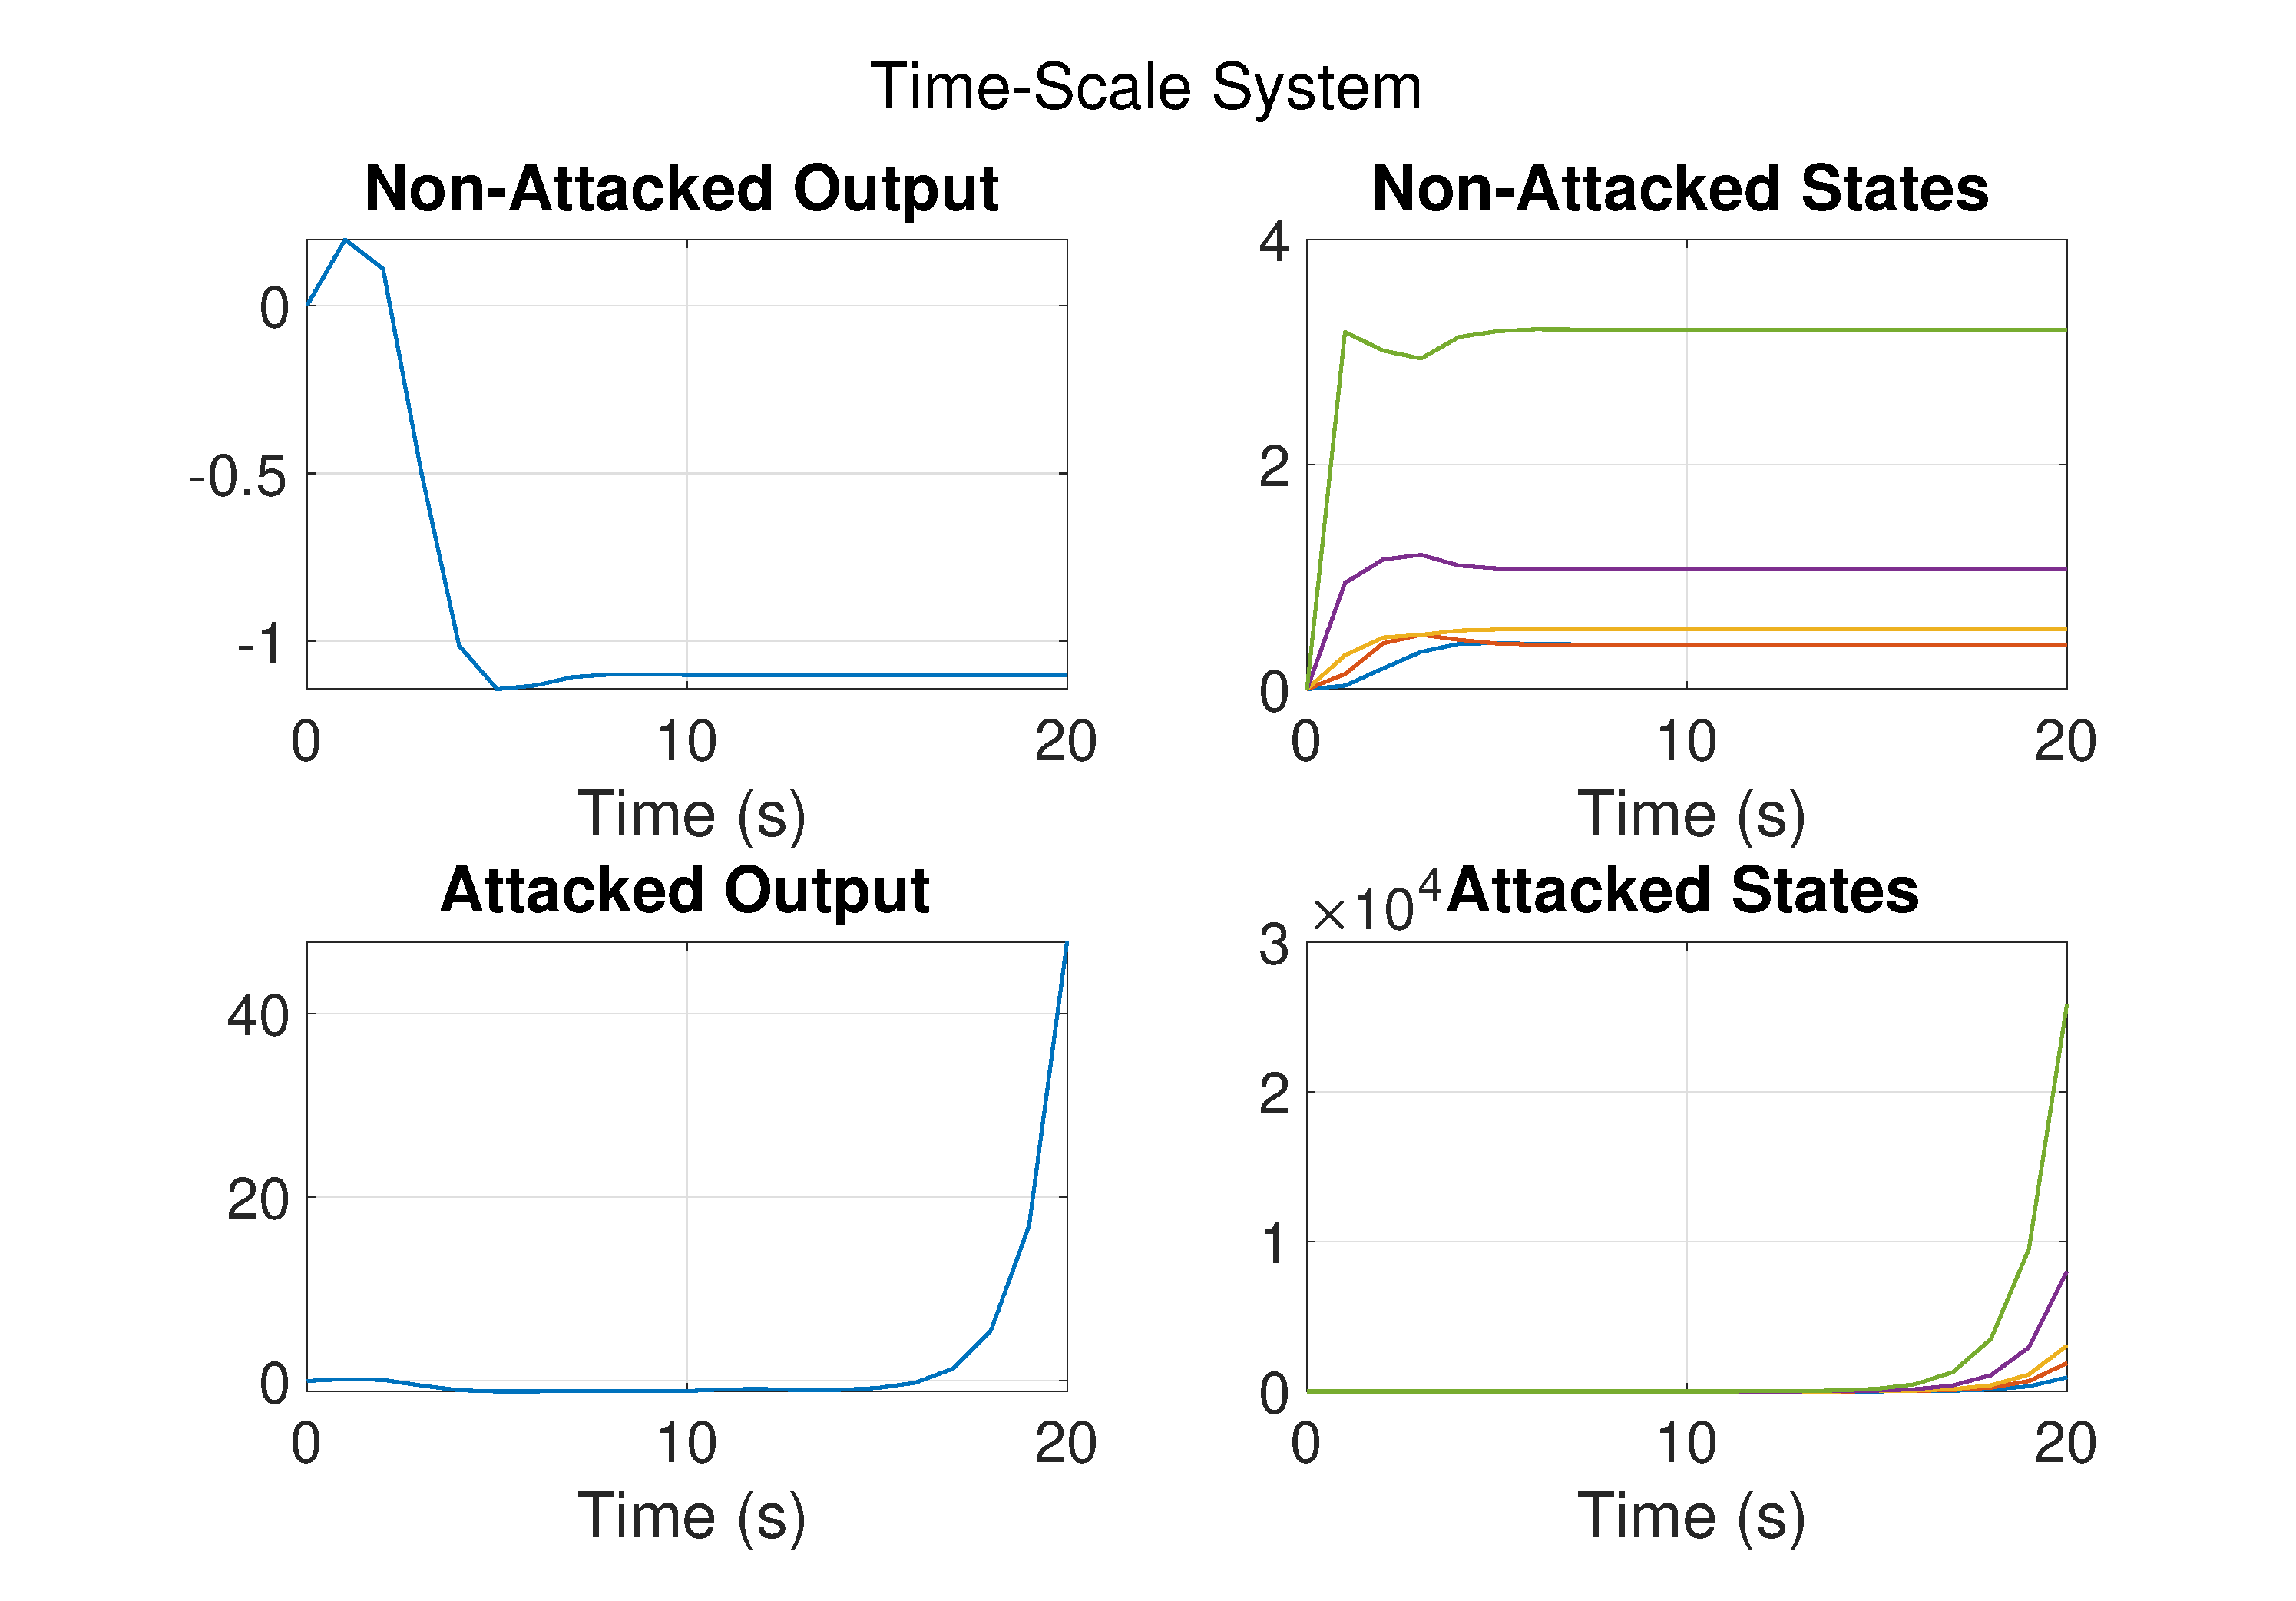
\includegraphics[width=\linewidth]{ts-system}
        \caption{Time-scale system's observer with \(\mu=\SI{1}{\second}\).}%
        \label{fig:ct-system}
      \end{figure}
    \end{column}%
    \hfill%
    \begin{column}{0.55\textwidth}
      \begin{figure}[ht!]
        \centering
        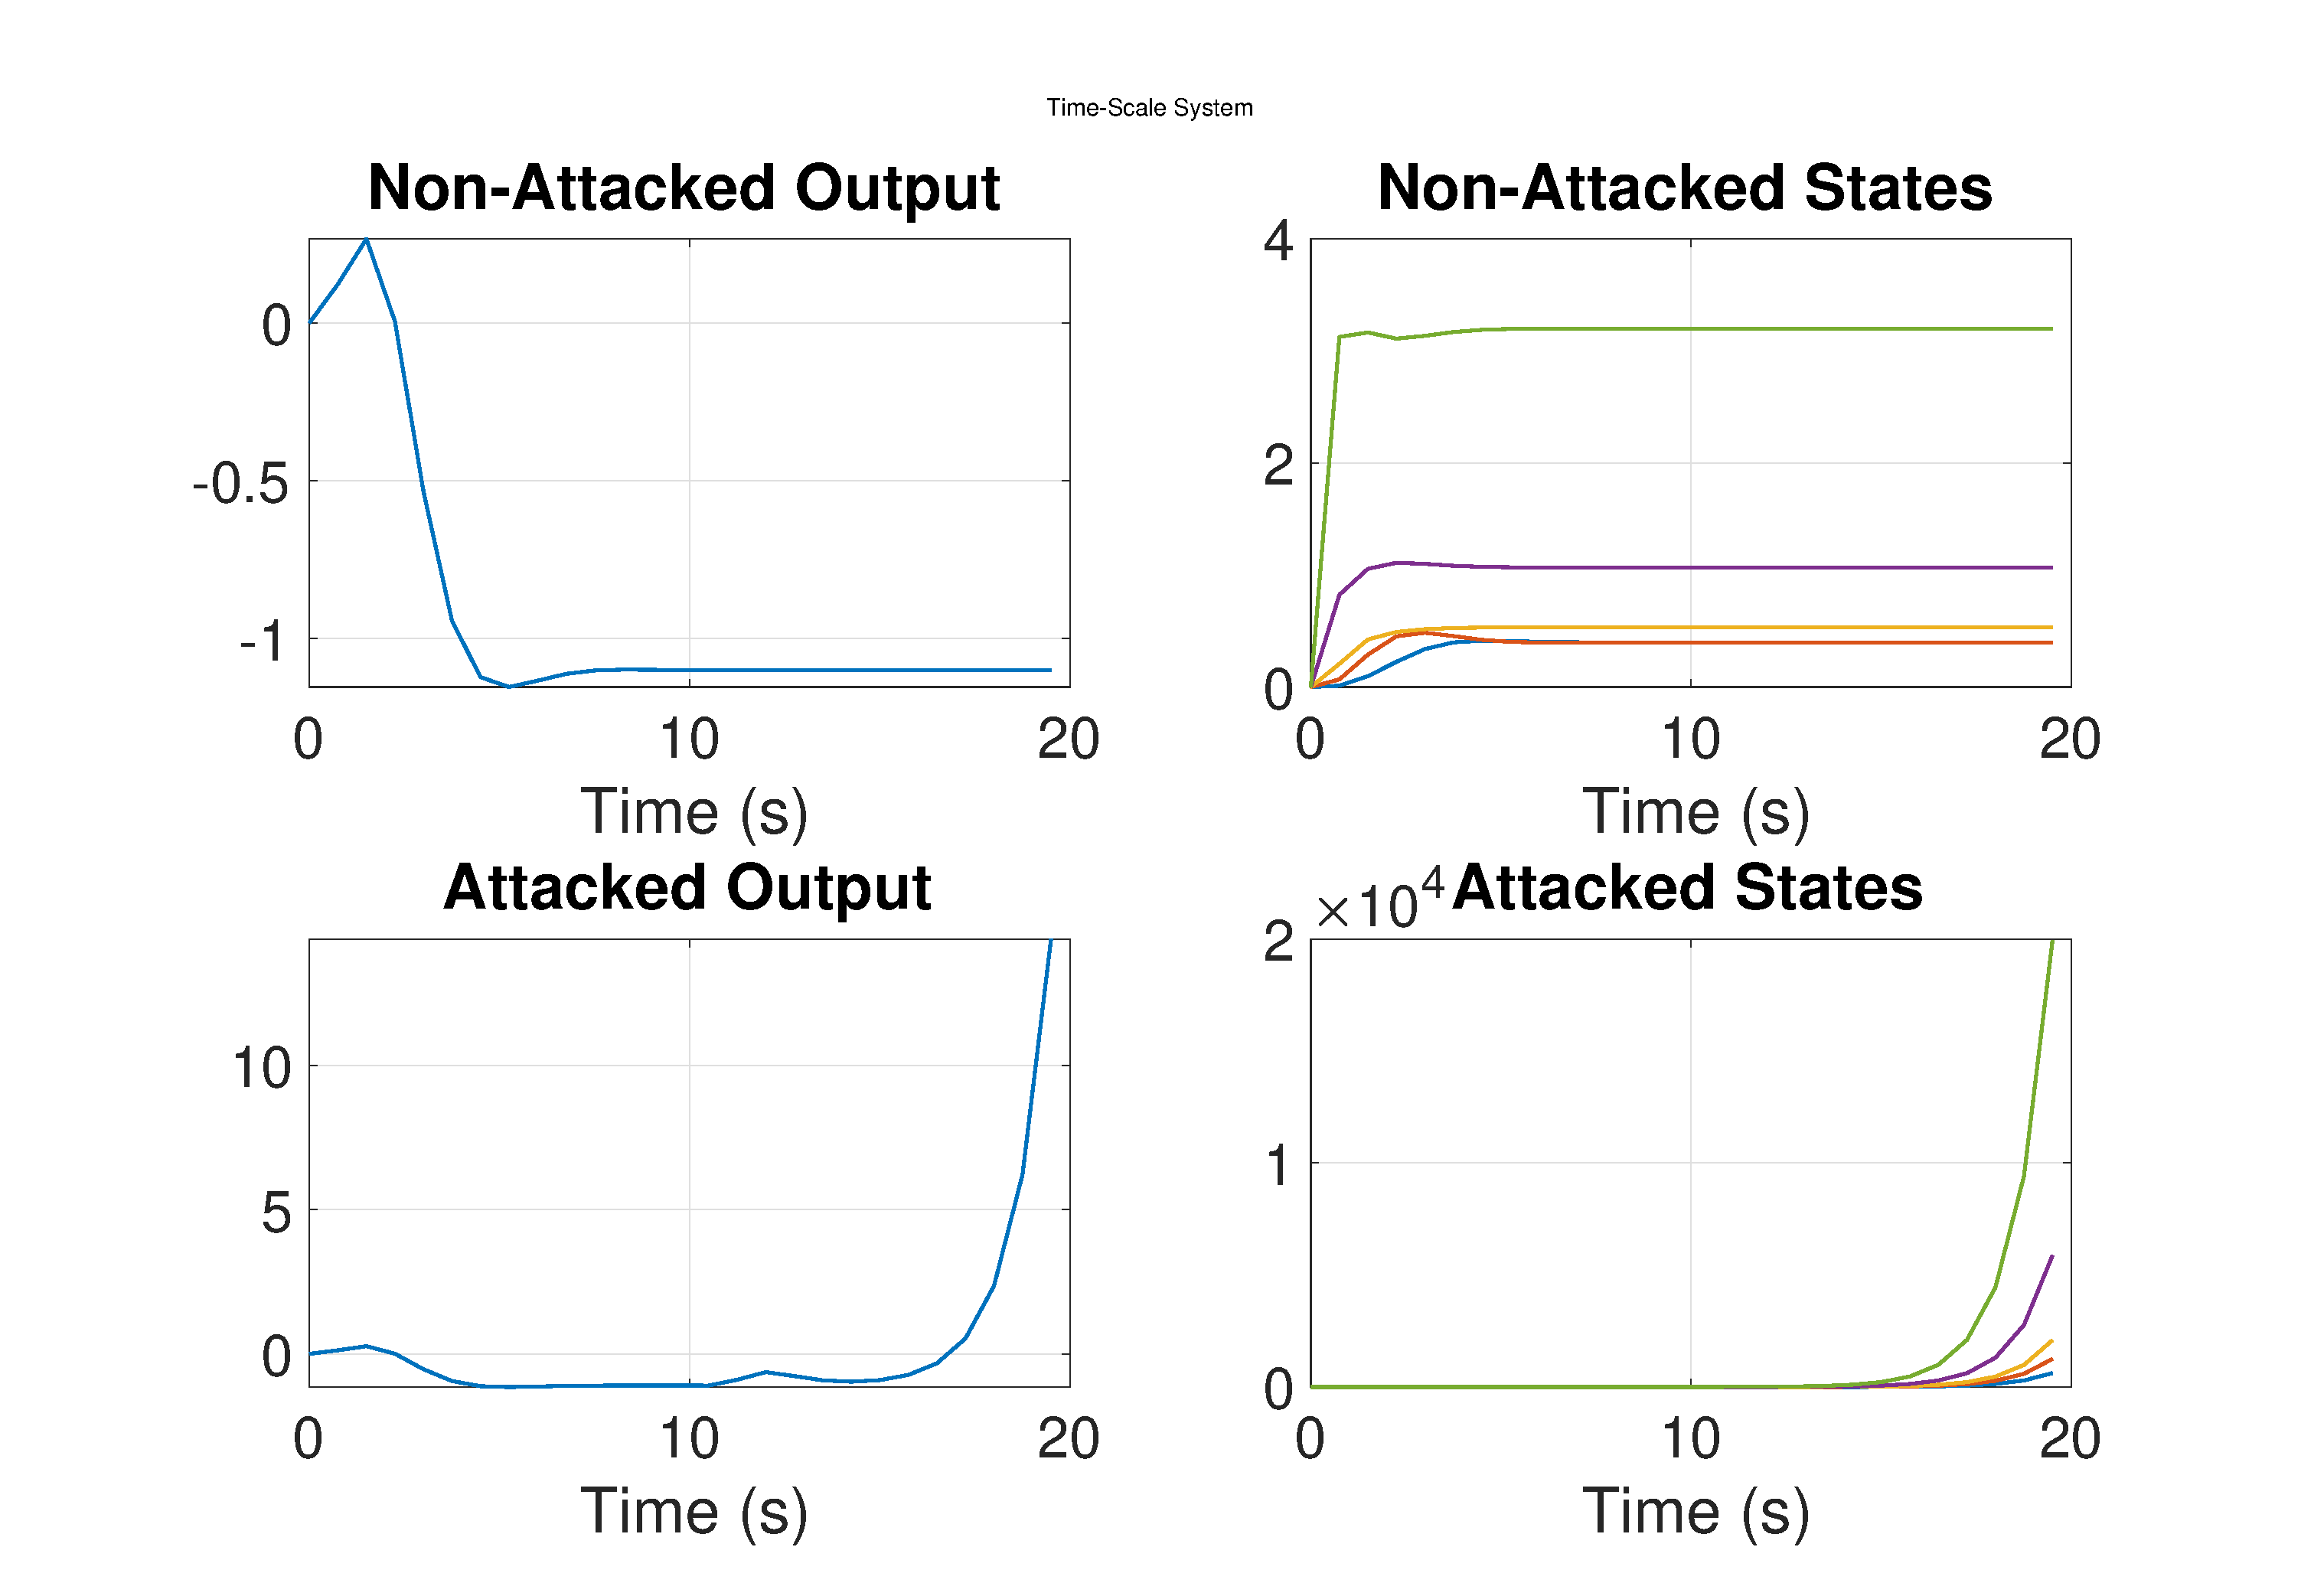
\includegraphics[width=\linewidth]{ts-system2}
        \caption{Time-scale system's observer with \(\mu=\SI{0.75}{\second}\).}%
        \label{fig:ts-system}
      \end{figure}
    \end{column}%
  \end{columns}
\end{slide}
